\section{Introduction}
In this chapter, we will define the performance metrics that are crucial to assess the effectiveness of the mobile multicast solutions. The performance metrics are typically based on such metrics for evaluation of a mobility management protocol as signaling cost, handover latency, and packet loss. Furthermore, the multicast-related metrics e.g., packet duplication, leave latency, end-to-end delay and tunneling overhead should be considered.

It is generally acknowledged that a proposed solution cannot be widely accepted without results from a valid experimentation, which can be obtained through various methods, each with its own advantages and limitations. Within the networking field of research, the results’ reliability is one of the most critical issues. Thus, the results' credibility is directly related to the methods used, therefore improving them becomes of great importance. In this context, the most widely used method - simulation - sometimes lacks credibility. The lesser used but most credible method - real testbed - is too expensive and difficult to scale and manage. In this chapter, we propose a \textit{hybrid} method which is a combination of virtualization and simulation. Through the study of a simple use-case showing mobility with PMIPv6, we demonstrate that our proposed method provides realistic results at a low cost. In other words, the near-to-real results can be achieved even with limited resources.  This method can also be deployed in a distributed manner for increased scalability. Additionally, the others tesbted e.g., MIP, HMIP, and DMM can be deployed using the same method. 

Throughout this thesis, in order to validate the results, firstly, we will use an analytical analysis. The proposed experiment method then, in some cases, will be used to improve the degree of confidence of the results. It can be considered as a framework that aims to close the gap observed between the research experimentation and the real deployment.
 
\section{Performance Evaluation Metrics}
At first, we identify the key requirements that need to be satisfied by the proposed solutions. Respecting these requirements, we then define the performance metrics that are crucial to assess the effectiveness of the solutions.

\subsection{Specific System Requirements}
In this thesis, our objective is to deal with the multicast-related issues raised when a multicast node is on the move. In other words, the aim of this research is to find solutions that ensure:
\begin{itemize}
\item Keeping the MN unaware of mobility from the multicast service point of view;
\item Minimizing the service disruption to even satisfy the strict requirements for the interruption- and delay-sensitive services;
\item Keeping the signaling/tunneling overhead as low as possible;
\item Maximizing the available network resource (reducing the waste of resource and packet duplication), keeping the reliability and improving the scalability of the system;
\item Minimizing the modifications of the mobility management and the multicast routing protocols to support IP mobile multicast. 
\end{itemize}

Based on these objectives, we will design novel solutions addressing the IP mobile multicast issues in both PMIPv6 and DMM environment. In the following, a list of specific requirements that would lead to the design of the target solution is provided:
\begin{itemize}
\item Only the network-based mobility management shall be studied to keep the MN unaware of mobility and to avoid modifications required at the MN;
\item Network access technology independence and support for both single-homed (e.g., Wi-Fi or LTE) and multi-homed terminals (e.g., LTE and Wi-Fi) shall be provided. In other words, such a generic solution which does not depend on specific access technology shall be provided;
\item Buffering technique shall not be considered. However, it can be used later to improve the proposed solution;
\item The routing paths between sources and listeners shall be optimized;
\item Mobility services shall be enabled only for IP flows which really need service continuity.
\end{itemize}

\subsection{ Performance Evaluation Metrics for IP Mobile Multicast}
To evaluate the performance of a mobility management protocol, a set of metrics in general is considered including signaling cost (location update cost), handoff delay, end-to-end delay and packet tunneling cost \cite{HO_comparison_Makaya, HO_comparison_Lee,HO_comparison_Costa,RO_PMIPv6_Lee}.

In wireless mobile networks, the mobility anchor is responsible for tracking the location of the MN to provide the mobility support. 
Thus, location management is crucial for the effective operation of wireless networks \cite{movement_based_mobility}. Location update is done by exchanging the signaling messages between the MN and the network entities (or between the network entities). In this context, the signaling cost is defined as the cost to update the location of the MN. It can be considered as a function of different metrics as the hop distance between the entities, the unit transmission cost over wired/wireless link, and the handover rates (intra- and inter-domain handover), etc. Signaling cost is an important factor since it influences the scalability of the system as well as the cost for data delivery. This metric becomes even more critical with the presence of wireless links whose have a limited capacity.

Regarding the handoff latency, it is defined as a period when a node cannot receive/send the packets while performing a handover. It is the time that elapses between the last packet received via the old router and the arrival of the first packet via the new router after a handover. During this period, the packets will be lost. Thus, it may result in noticeable service disruption, especially in case of delay sensitive applications like video and Voice over IP (VoIP). The number of lost packets typically is proportional to the handover latency. In IPv6-based networks, QoS may be defined by packet loss, handoff latency and signaling overhead \cite{HO_comparison_Makaya}. As a result, long handover latency and a large number of lost packets may degrade the quality of service. Thus, reducing the handover latency and the packet loss enhances the performance of user applications. 

On the other hand, the end-to-end delay between two nodes is the summation of delays experienced along the path between these nodes. In general, the end-to-end delay consists of not only the transmission delay over the links but also the queuing and processing delay at the intermediate nodes \cite{e2e_delay_Li}. Many popular multimedia applications, e.g., real time gaming, live video streaming, and conversational VoIP/Video, have strict delay requirement. 

Regarding IP mobile multicast, the similar metrics as mentioned as above as well as the multicast-related metrics should be taken into consideration. 
\subsubsection{Signaling and Packet Delivery Cost}
The signaling cost is the signaling overhead for supporting the handover of a multicast node, including the cost for the location update and the multicast-related procedures. It is defined as the total delivery cost of all signaling messages. According to \cite{RO_PMIPv6_Lee}, the signaling message delivery cost is calculated as the product of the message size, the hop-count distances and the unit transmission cost over wired/wireless link. Let $\alpha$ and $\beta$ denote the unit transmission cost for the wired and the wireless link, respectively. Thus, the signaling message delivery cost over the wired link from node X to node Y is calculated as\\
\begin{equation}
SMC_{wd} = \alpha l  h,
\end{equation}
where $l$ is the size of the message, $h$ is the hop distance between X and Y. In case of wireless link, the message delivery cost can be expressed as
\begin{equation}
SMC_{wl} = \beta  l h.
\end{equation}

Note that typically the hop-count distance between two nodes via wireless link is 1. In some cases, for the sake of simplicity, the size of signaling messages is considered as identical. In this case, this value can be included in the parameters $\alpha$ and $\beta$. 
The signaling cost, as the accumulative signaling overhead, can be calculated as
\begin{equation}
SC = \sum_{all} SMC.
\end{equation}

On the other hand, the packet delivery cost represents the accumulative cost to deliver multicast packets from the source to the listener per unit of time. It is proportional to the distance between the source and the listener, the size of data packets and the number of packets transmitted. 

\subsubsection{Multicast Service Disruption Time and Packet Lost}
The multicast service disruption time ($SD$) is defined as a period when a multicast listener/source cannot receive/send the multicast packets. It is calculated as the total time needed to complete the mobility handover and the multicast-related procedures. Thus, the multicast service disruption time typically consists of: i) Layer 2 handover duration ($t_{L2}$) which is the reattachment time from the previous point of attachment to the new one. It depends on specific wireless access technology, for example, in case of 802.11 WLAN its includes the time for channel scanning, authentication, and association/re-association process; ii) Layer 3 duration ($t_{L3}$) caused by IP-related procedures; and iii) The delay due to the multicast-related procedures, called $t_{M}$. $t_{M}$ is defined as the total time taken to complete all the multicast-related procedures including the multicast knowledge gain, multicast subscription and transmission time for the first multicast packet from the multicast router to the listener after handover. As a result, the multicast service disruption time is defined as 
\begin{equation}
SD = t_{L2} + t_{L3} + t_{M}.
\end{equation}

To calculate the layer 3 and the multicast handover delay, we adopt the packet transmission delay model in \cite{packet_transmission_delay}, in which the packet transmission consists of the transmission time and the propagation time.  
According to \cite{packet_transmission_delay}, the transmission delay of a wired link can be calculated as\\
\begin{equation}
d_{wd}(l,h) = h (\dfrac{l}{BW_{wd}} + D_{wd}),
\end{equation}
where $h$ is the hop-count distances between two nodes, $l$ is the length of the packet, $BW_{wd}$ is the bandwidth of the wired link and $D_{wd}$ is the wired link latency. 

Unlike the wired transmission which can be considered as reliable, the wireless link is unreliable. Thus, the probability of link failure should be taken into account. The wireless transmission delay therefore is given by \cite{packet_transmission_delay}\\
\begin{equation}
d_{wl}(l) = \dfrac{1}{1-q} (\dfrac{l}{BW_{wl}} + D_{wl}),
\end{equation} 
where q is the probability of the wireless link failure, $BW_{wl}$ is the bandwidth of wireless link and $D_{wl}$ is the wireless link latency.  

For a sake of simplicity, the transmission delay in some cases can be considered as proportional to the distance, for example, with the proportion is $\tau$ for wired link and $\kappa$ for wireless link. Thus, the transmission delay is simply given by
\begin{equation}
d_{wd}(h) = \tau h,
\end{equation}
\begin{equation}
d_{wl} = \kappa.
\end{equation} 

On the other hand, the packet loss ($\varphi_{p}$) represents the number of lost packets during handover. Typically, the number of lost packets is proportional to the service disruption time and the packet arrival rate. As a result, it is given by
\begin{equation}
\varphi_{p} = \lambda_{p} SD,
\end{equation} 
where $\lambda_{p}$ is the packet arrival rate.

\subsubsection{End-to-End Delay}
As stated earlier, the end-to-end delay consists of not only the transmission delay over the links but also the queuing delay and the processing delay at the intermediate nodes. However, for a sake of simplicity, the queuing delay as well as the processing delay are supposed to be small enough to be ignored in the performance analysis. As the result, the end-to-end delay represents the packet transmission delay from the source to the listener. The packet transmission consists of the transmission time and the propagation time. It is proportional to the distance between two nodes, the size of the packets, the bandwidth of the link and the link latency \cite{packet_transmission_delay}. Typically, the packet transmission delay over a wired and a wireless link is different. 
\subsubsection{Other Metrics}
In addition to the above-mentioned metrics, those as packet duplication, tunneling overhead, waste of resource, scalability, and easy-to-deploy should be taken into consideration. In the context of our thesis, the scalability issue will be considered in terms of load balancing among LMAs (together with the signaling cost). The packet duplication metric reflects the tunnel convergence problem. 

\section{Experimental Evaluation of Wireless Mobile Network}
In networking research, there are various experiment methods such as: using a real testbed, simulation, emulation, virtualization and mathematical or theoretical modeling. Each method has its own advantages and limitations \cite{art_of_analysis}. Using a real testbed is considered as the best experimental method. It implies, however, a higher cost of deployment and lack of scalability. Although simulation is quite popular thanks to its flexibility and easy-to-deploy features, the results obtained in some cases are not reliable. Emulation can be considered as a trade-off between simulation and a real testbed bringing more accurate results (compared to simulation) and lower cost (compared to the real testbed). Yet, emulation has limitations on deployment and scalability, which can be mitigated by using the technique of machine virtualization.  Finally, mathematical modeling is sometimes used, but only in a simplified way, abstracting most of the complexity and reflecting it on obtained results. Furthermore, to help justify our approach on experimental method, we must mention that our case study concerns mobile environments and therefore we must keep in mind the most important requirements that an experimental method must focus on are accuracy, reliability, mobility, and scalability \cite{ASSERT}. 

In this section, we introduce a near-to-real experiment environment which consists of a virtualized and simulated environment. The first part can be considered as the network infrastructure in which multiple virtual machines are connected together, while the second part is a wireless access network mainly composed by a wireless simulator. By combining these components we produced a method that can achieve a higher level of realism while keeping the advantages of the simulation method and still be able to run real software and real world protocols. Since this experiment environment is an open-source and easy to deploy, it can be reused by other researchers to set up their own experiment environment. Additionally, it allows the design and evaluation of small to medium scaled networks and deployed protocols whose results can be easily translated to the real world. These characteristics will be illustrated through the analysis of our case study using PMIPv6 \cite{PMIPv6}. Particularly, this method is suitable for following cases: i) fixed infrastructure; ii) mobility and mobile networks; iii) network and upper layer experimenting (e.g. mobility management, multicast, applications, etc.); iv) up to medium sized infrastructure networks; and v) large sized networks of mobile nodes.

\subsection{Experiment Methods in Networking Research}
This subsection introduces the most relevant experimental methods in the field of networking research, emphasizing their advantages and disadvantages. We start by the most popular method, simulation, and then move to real testbeds, emulation and mathematical modeling. We continue by addressing the required criteria to our work, which is supported by acknowledged good practices on credibility and confidence of experimental methods.  

Simulation is the most common experimental method in networking research \cite{MANET_simulation} \cite{case_study_simulation}, mainly due to the fact that simulation environments can provide large-scale flexible scenarios (in terms of topology, number of nodes) at a low cost. In addition, the capability of reliable reproduction and repetition of experiments is embedded. However, the main drawback of this method is the lack of credibility \cite{credibility_simulation,improving_confidence}. In other words, the results of the simulation in some cases cannot be relied on, particularly for mobile network experiments, due to the complex environment of mobile wireless networks and the simplicity of the simulation framework. The varying degree of simplification has allowed the creation of several simulators for mobile wireless networks e.g., OMNet+++, Matlab, Glomosim (QualNet), NS-2 and NS-3. Each simulation tool has its own advantages and limitations \cite{case_study_simulation}. The choice of a simulation tool depends on several factors such as cost, ease of use, level of complexity, availability of required model, community support, and particularly accuracy. Regarding accuracy, the results may be very different when using different simulation tools \cite{accuracy_MANET}, making it difficult to choose the appropriate simulation tool.

On the other extreme of the experimental methods is the construction of a real testbed which uses a set of real hardware and software. In general, it is considered the best environment for experiment study, since this kind of method provides the most accurate and most realistic results \cite{real_testbed_Montavont}. Furthermore, it helps to find unexpected errors and limitations that could not otherwise be observed in the simulation. However, this method requires a high cost especially when a complex network topology and a large-scale experiment are considered. Also, additional effort may be required when considering the mobility of the nodes (e.g., unpredictable and hard to repeat, scaling of the geographical movement, mobility pattern and experiment management). The repeatability and reproducibility also present some serious challenges.  

In the middle of the extremes, emulation has been introduced as a compromise between these two above-mentioned methods. The main advantage of this approach is that it helps to eliminate the practical problem with the real testbeds by completely controlling such external factors that may influence the experiment thus increasing repeatability and reproducibility. It can also provide the near-to-real results at a lower cost in comparison with the real testbed. However, the emulation experiment may still lack scalability and its not always easy to set up an emulation environment. Another possible method is the virtualization in which a whole network is created by the virtual machines. The advantage of this method is that the development of the software can be done on the real machine, tested on the virtual network of virtual machines, and later installed without any  (or with minor) modifications on the real testbed. However, virtualizing wireless network interfaces as well as simulating mobility of the nodes are complex tasks \cite{virtual_WiFi, LTE_virtualization}. The oldest method is theoretical modeling with mathematical analysis, which uses a mathematical model to evaluate network performance. However, it is very difficult to model a realistic environment particularly in the case of mobile wireless networks. As a result, some simplifications are required. 

Regarding one of the most important issues – credibility, in \cite{credibility_simulation}, the authors raised the credibility issue over a survey of over 2200 publications in the field of network simulation studies. They provided some guidelines to help to ensure a basic level of credibility of simulation experiments such as: i) the simulation experiments should be repeatable; ii) the method of analysis of simulation output data should be specified; and iii) the final statistical errors associated with the results should be provided. In conclusion, ideally, an experimental method would focus on some requirements such as controllability, repeatability, cost effectiveness, data collection, resource sharing, and particularly elements such as scalability, accuracy and mobility \cite{ASSERT}, are at the core of the trade-off or compromise that leads the researcher to choose his experimental method.

\subsection{Virtualization Technique and Virtual Networking}

In this section, we introduce our approach and the different techniques considered for virtualization as well as the tools for virtual networking. We then focus on the tools that help to deploy the virtual networking such as Virtual Network User Mode Linux (VNUML)\footnote{VNUML Homepage: http://www.uni-koblenz.de/~vnuml/index.en.php}, and Netkit\footnote{Netkit Homepage: http://wiki.netkit.org/} regarding their advantages and their limitations.  
\begin{figure}[tb!] 
  \begin{center} 
    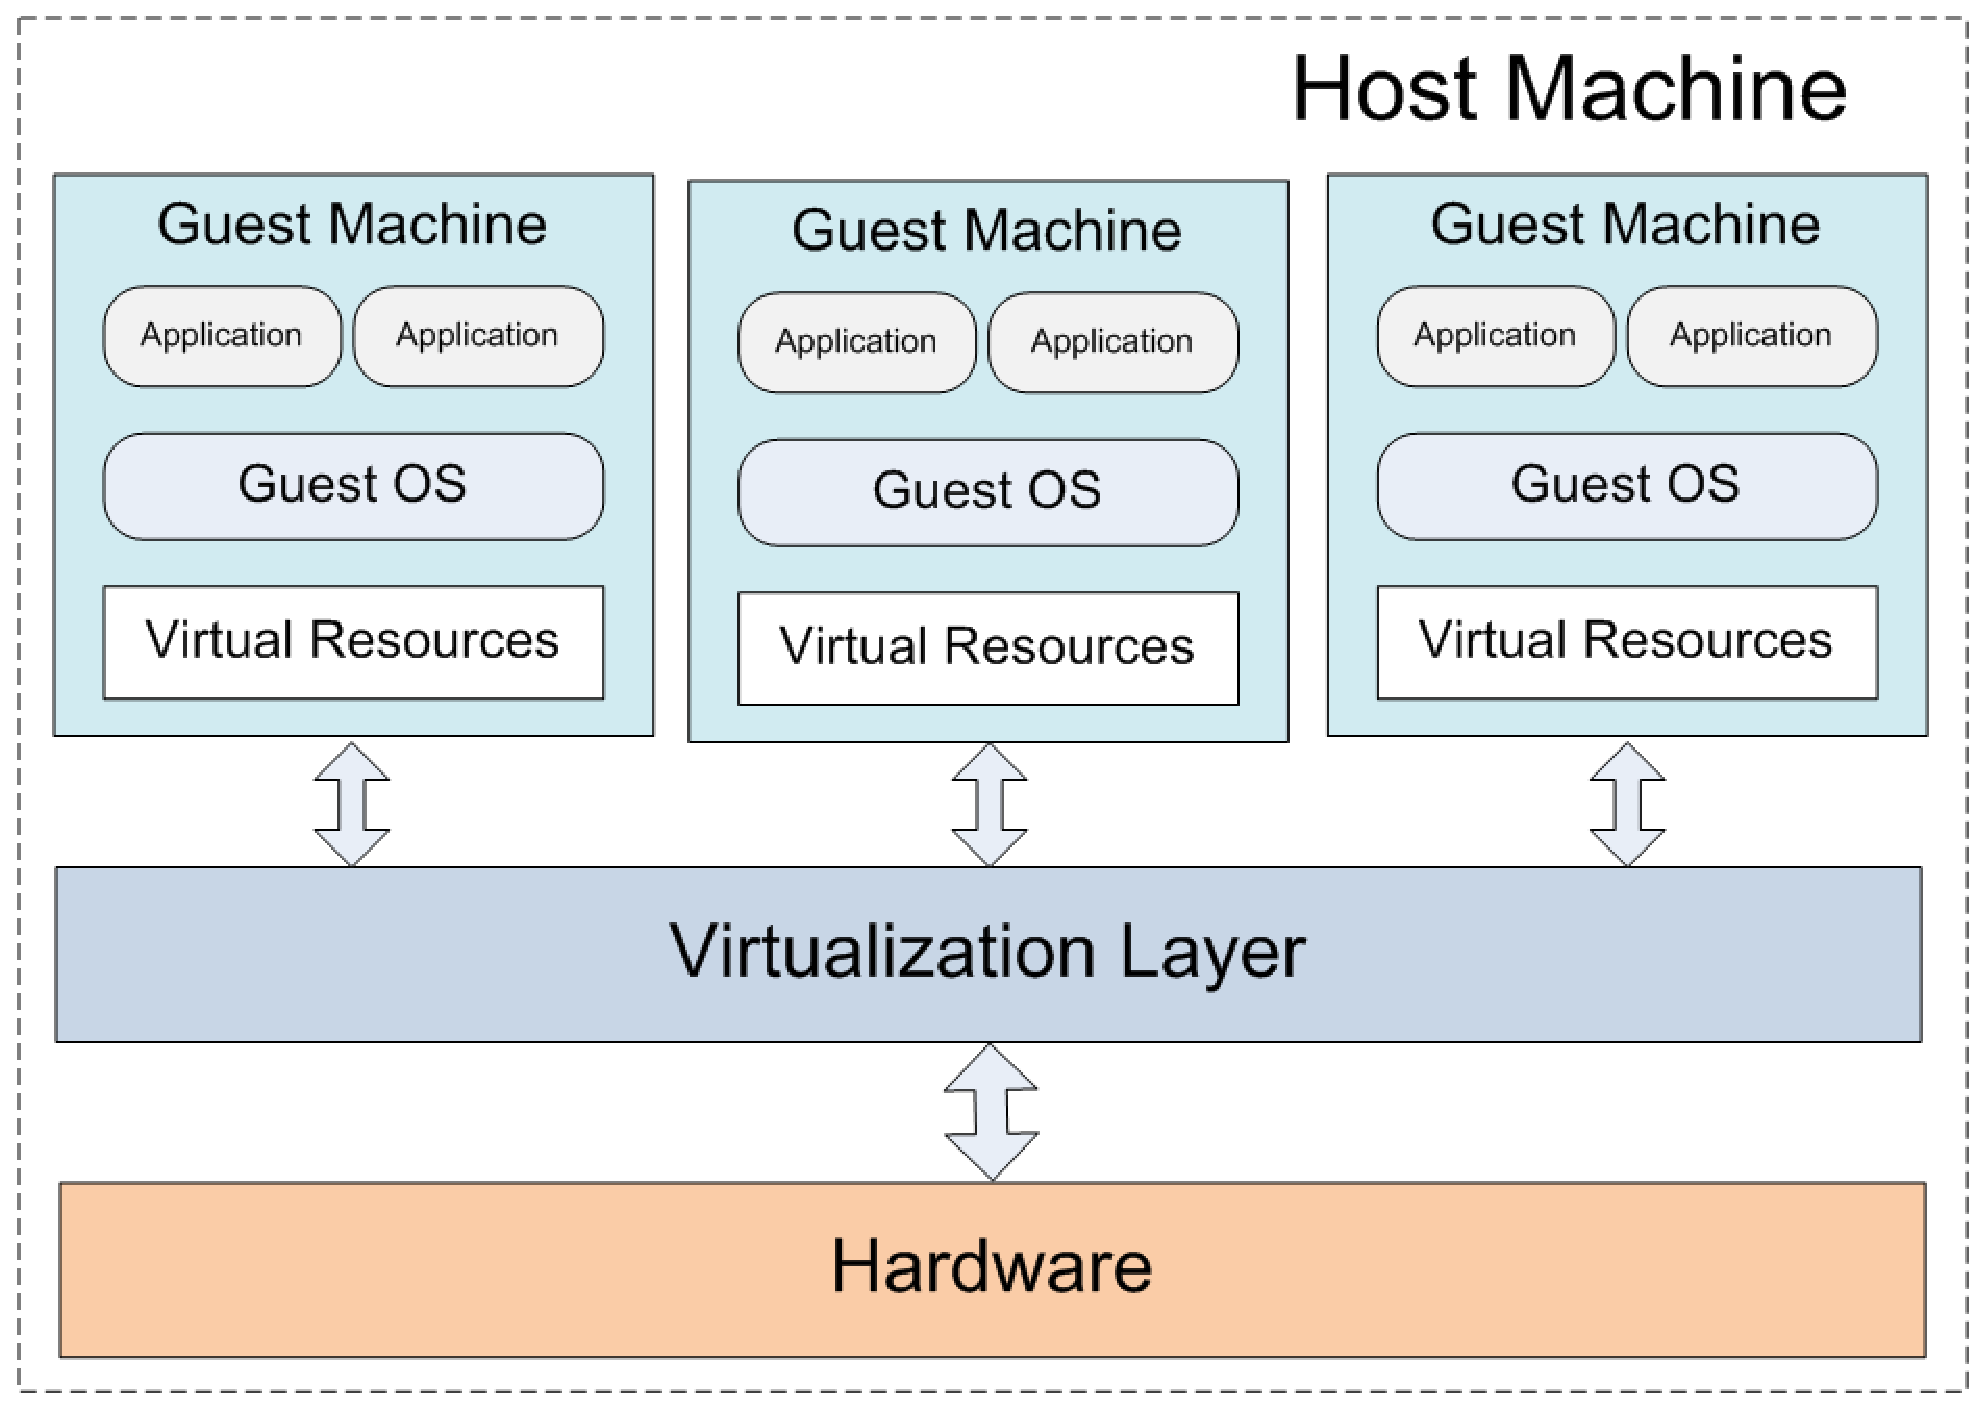
\includegraphics[width=0.55\textwidth]{./Part1/Chapter3/figures/c5_virtualization_technique.eps} 
    \caption{An example of the virtualization technique.}
    \label{fig:c5_virtualization_technique}
  \end{center} 
\end{figure}  

\subsubsection{Virtualization Techniques and Virtualization Tools}
Virtualization is a mechanism which allows running multiple independent and simultaneous instance sets, of the machine’s core software components (such as kernel, memory management, etc.), creating in practical terms a framework where these instance sets constitute the virtual logical machines (guest machines), which, when executed will share the physical resources of the single physical machine (host machine) \cite{virtualization_concepts, VMWare_whitepaper}. Since several virtual machines can be run inside a limited resource, then a virtual environment can help to extend the capabilities of a system at a low cost. Fig.~\ref{fig:c5_virtualization_technique} shows an example of virtualization technique. In this figure, the different guest machines run on the real machine. The guest machines use the virtual resources which are mapped to the sharing physical resources of the host machine (e.g., CPU, storage, and memory). The allocation and sharing of these resources is managed by the virtualization layer.

There are several virtualization techniques depending on the way the virtualization layer is implemented, the first technique is full virtualization (using binary translation) \cite{VMWare_whitepaper} in which the guest operating system (OS) acts as if it owned the hardware. That means the guest OS does not know that it is being virtualized and as a result, the guest OS does not require any modification. However, an additional mechanism, namely binary translation, is required to trap the instructions that are not compatible with the virtualization (non-virtualized) and translate them into the new instructions that will have the same effect on the virtual hardware. Some examples of the full virtualization technique are VMWare\footnote{VMWare Homepage: http://www.vmware.com/}, and Virtual Box\footnote{Virtual Box Homepage: https://www.virtualbox.org/}. 

The second technique is paravirtualization (or OS assisted virtualization) \cite{VMWare_whitepaper}. Unlike the full virtualization technique, the guest OS is aware of the fact that it is running in a virtualized environment. Thus, the guest OS is modified from the standard OS to communicate directly with the virtualization layer in case of non-virtualized instructions. Thanks to this mechanism, the paravirtualization achieves better performance than the full virtualization. However, one of the main drawbacks of the paravirtualization is that it fails to support any OS which is unprepared for virtualization. The paravirtualization is, for instance, supported by Xen \cite{Xen} and User-mode Linux (UML) \cite{UML}, etc. 

The last main virtualization technique is called hardware-assisted virtualization (or native virtualization) \cite{hardwared_assisted}. This technique requires the hardware to support the virtualization technology in order to simplify the virtualization mechanism. Since this technique is quite new, at this stage, it can only bring advantages in some limited cases \cite{VMWare_whitepaper}, though its results look very promising. Kernel Virtual Machine (KVM)\footnote{Kernel Based Virtual Machine (KVM) Homepage, http://www.linux-kvm.org/} is an example of the hardware-assisted virtualization. 

When considering different virtualization tools in the context of network environment, a lightweight tool should be chosen in order to deploy as many virtual nodes as possible in a single physical machine. In this context, this chapter adopts UML since it is a relatively lightweight technique compared to the others \cite{evaluation_UML}. UML is also one of the most popular virtualization techniques that can be deployed in a linux-based OS.

UML uses the paravirtualization technique (at kernel level) that allows running a virtual instance of Linux inside the host Linux OS as a normal system process. In these conditions, a virtual machine running with a UML kernel (modified kernel) and a root filesystem, can be assigned to the virtual resources and have a hardware configuration entirely separated from that of the host. 

\subsubsection{Virtual Networking in Linux}
As mentioned above, there are many virtualization techniques. However, some may require a number of manual operations to set up a virtual network and interconnect virtual machines. That is why there are several tools which aim at building and configuring a virtual network environment easily and automatically. They are developed to simplify this task (such as VNUML, Netkit, and Marionnet\footnote{Marionnet homepage: http://www.marionnet.org/EN/}, which rely on UML) and allow to design and test networks with different topologies and different configurations. The created virtual networks are able to communicate with both the host machine and, if possible, with any existing network connections residing on the host. 
Nevertheless, there are several limitations in the context described in this chapter:
\begin{itemize}
\item \textit{Centralized deployment}: That means the entire virtual network is deployed inside just one host machine which limits the deployment size since resources are shared. 
\item \textit{No wireless access technology support}: They fail to support wireless access connections such as WLAN, and LTE, since their deployment only considers static point-to-point connections.
\item \textit{Difficult to support different kernels and filesytems overall network}: Typically, only one kernel and filesystem are used for all the virtual machines. In some case, due to the conflict between the software requirements, it is impossible to use only one kernel version with the same components installed for all the network entities. Moreover, one configuration for all machines is not always a good option, e.g., the servers require much more resources than the mobile nodes. Also, while servers may require some additional software, mobile nodes do not.
\end{itemize}

\subsection{Wireless Simulation and Emulation}
In reality, there are various wireless simulation tools (e.g., OMNet+++, Matlab, Glomosim, NS-2 and NS-3), with each tool having its own advantages and limitations. Thus, choosing an appropriate tool is very difficult since it can lead to unexpected results which cannot be exploitable in a real world deployment. 

In this subsection, we also look at simulation tools which can provide the wireless emulation mode such as NS-2, NS-3. With such a tool included in our work, real and virtual machines can be connected via an emulated wireless connection. Since NS-3 is relatively new and intended to replace the aging NS-2 simulator, it has a good development momentum which incorporates a remarkable number of interesting features \cite{NS-3-goal}. Those are the reasons why we selected NS-3 as the main tool to provide the emulation of wireless environment for the proposed testbed.

NS-3 is a discrete-event network simulator targeted for research and education. It relies on C++ and can be installed on common operating systems e.g., Linux, Windows, Mac OS. Furthermore, NS-3 provides an effective tracing method, called callback tracking system \cite{NS-3-goal}. By using this technique, a reaction can be executed when a trace source generates a new event, for example, for cross-layer interaction, statistic collection, etc. Beside the traditional text file as the output of events, NS-3 provides another type of tracing called PCAP (network traffic capture) which then can be used by a network analyzer tools e.g., Wireshark \cite{Wireshark}, Tcpdump \cite{Tcpdump} to analyze the results.

In addition to the simulation capability of NS-3, the emulation is natively supported by using a type of virtual network device, named Tap Bridges. Thus, the real services/nodes can communicate with the NS-3 environment. This capacity allows deploying a \textit{hybrid technique} as we used to develop the proposed testbed. 

\subsection{Requirements and Proposed Strategies}
\subsubsection{Requirements for a Wireless Testbed}
Regarding the experiments in the context of mobile environments (focusing on the network and upper layers), there are some requirements briefly described as follow. 

The first and the most important requirement is that the results of the experiment have to go in line with that from a real experiment. In other words, the experiment environment has to be able to provide realistic and reliable experiments. Then, the experiment environment should be able to emulate the mobility of several nodes by using a mobility pattern. Also, the flexibility in terms of network topology and mobility scenarios should be provided. The experiment environment should be reproductive, repeatable, and scalable in terms of number of network nodes, and it is important to use the virtualization tool that consumes fewer resources. Last but not least, the tools to collect and analyze results should be available and easy to use. Based on these requirements, a testbed environment is proposed as described in the following subsection. 

\subsubsection{Description of the Proposed Testbeds}

\begin{figure}
\centering
\subfloat[]{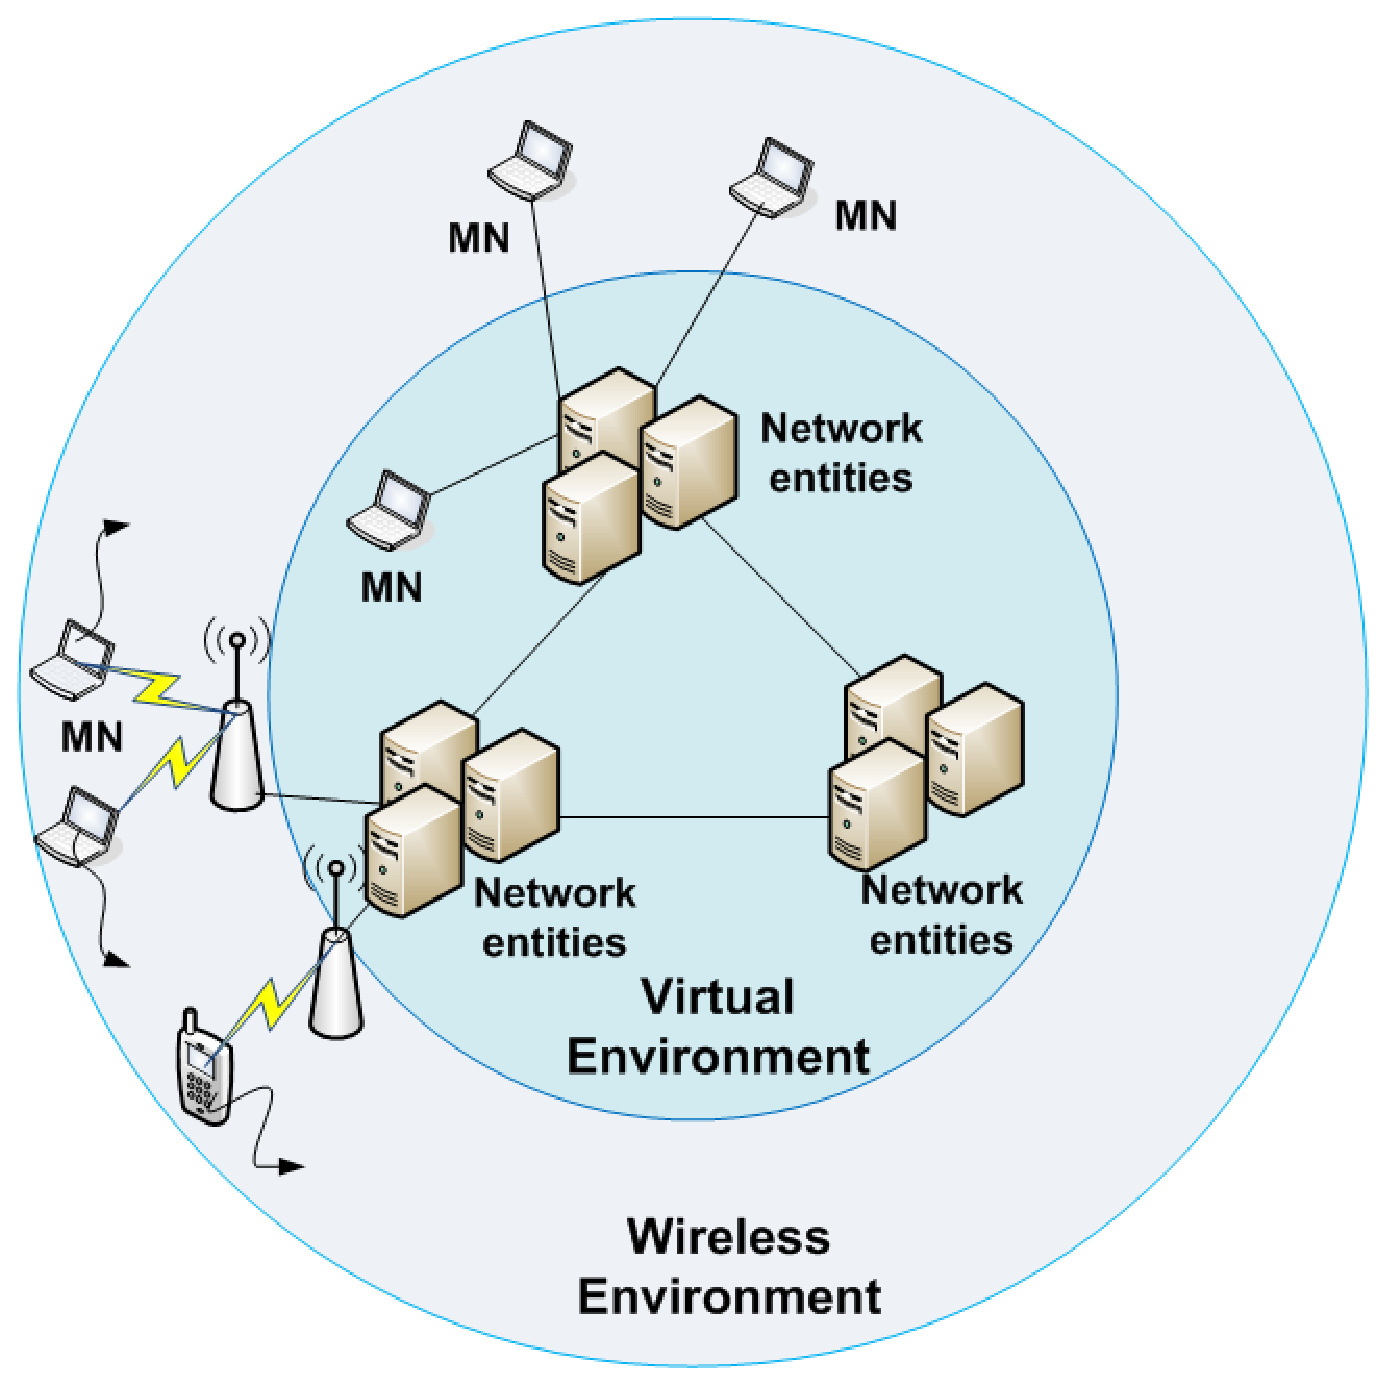
\includegraphics[width=0.40\textwidth]{./Part1/Chapter3/figures/c5_architecture.eps} \label{fig:c5_architecture}}\,\,\,\,\,\,
\subfloat[]{\includegraphics[width=0.48\textwidth]{./Part1/Chapter3/figures/c5_connection.eps}\label{fig:c5_connection}}
\caption[Architecture of the near-to-real testbed.]{Testbed Architecture: (a) Description of the testbed. (b) Connection between components.}
\label{scenariocbf}
\end{figure}

Due to the limitations of the above-mentioned methods and the requirements for the wireless experiment, we provide an ultimate method using a near-to-real testbed - a combination of a virtualized and a simulation environment, as depicted in Fig.~\ref{fig:c5_architecture}. This method allows keeping the results close to the real experiment without significant efforts. It also provides a flexible simulation in terms of network topology, and mobility scenarios. This method also potentially allows the medium-scale networks in term of infrastructure nodes and large-scale in terms of mobile nodes.

A main drawback of using UML for a wireless experiment is that it only offers a virtual Ethernet interface (not a virtual wireless interface), which is why we propose a combination of an UML-based virtualized network and a wireless simulator to provide a wireless experiment environment.

In this approach, the first part of the proposed environment consists of the virtual machines connected together. It represents the network infrastructure. The second part provides the wireless environment by using NS-3 (access points (APs) and mobile nodes). A network analyzing tool (e.g., Wireshark) as well as PCAP trace file can be used to capture the network traffic between the virtual machines. We can then analyze the track files to obtain the results.

Regarding the first part, as seen in Fig.~\ref{fig:c5_connection}, testbed environment is created by using the Linux bridge technique that allows connecting the virtual machines with the wireless interfaces present in the simulation environment. The virtual machines can be distributed among the different physical machines. However, a bit more effort is needed to create the network and experiment scenarios, in this example, we use a simple script. By using a virtual device (called TUN/TAP \cite{tun_tap}), the VM can communicate with the physical networking infrastructure as well as other VMs. TAP device works at the Ethernet frame level while TUN device acts as a network layer device. Similarly, a machine inside NS-3 can be made similar to a real machine thanks to the TapBridge mechanism\footnote{Tap Bridge Model NS-3: https://www.nsnam.org/doxygen/classns3\_1\_1\_tap\_bridge.html/}. 

Regarding the second part, NS-3 is used to emulate the wireless environment and the mobility of mobile nodes. With NS-3, heterogeneous access networks can be provided e.g., WLAN, WiMAX and LTE. In addition, the mobile node's mobility pattern (inside NS-3 e.g., random walk, random waypoint, random direction, and Gauss-Markov mobility model) and external mobility pattern can be used to allow simulating flexible, more realistic mobility of the nodes. 

\subsection{Tesbed Deployment}

\begin{figure}[h!]
\centering
\subfloat[]{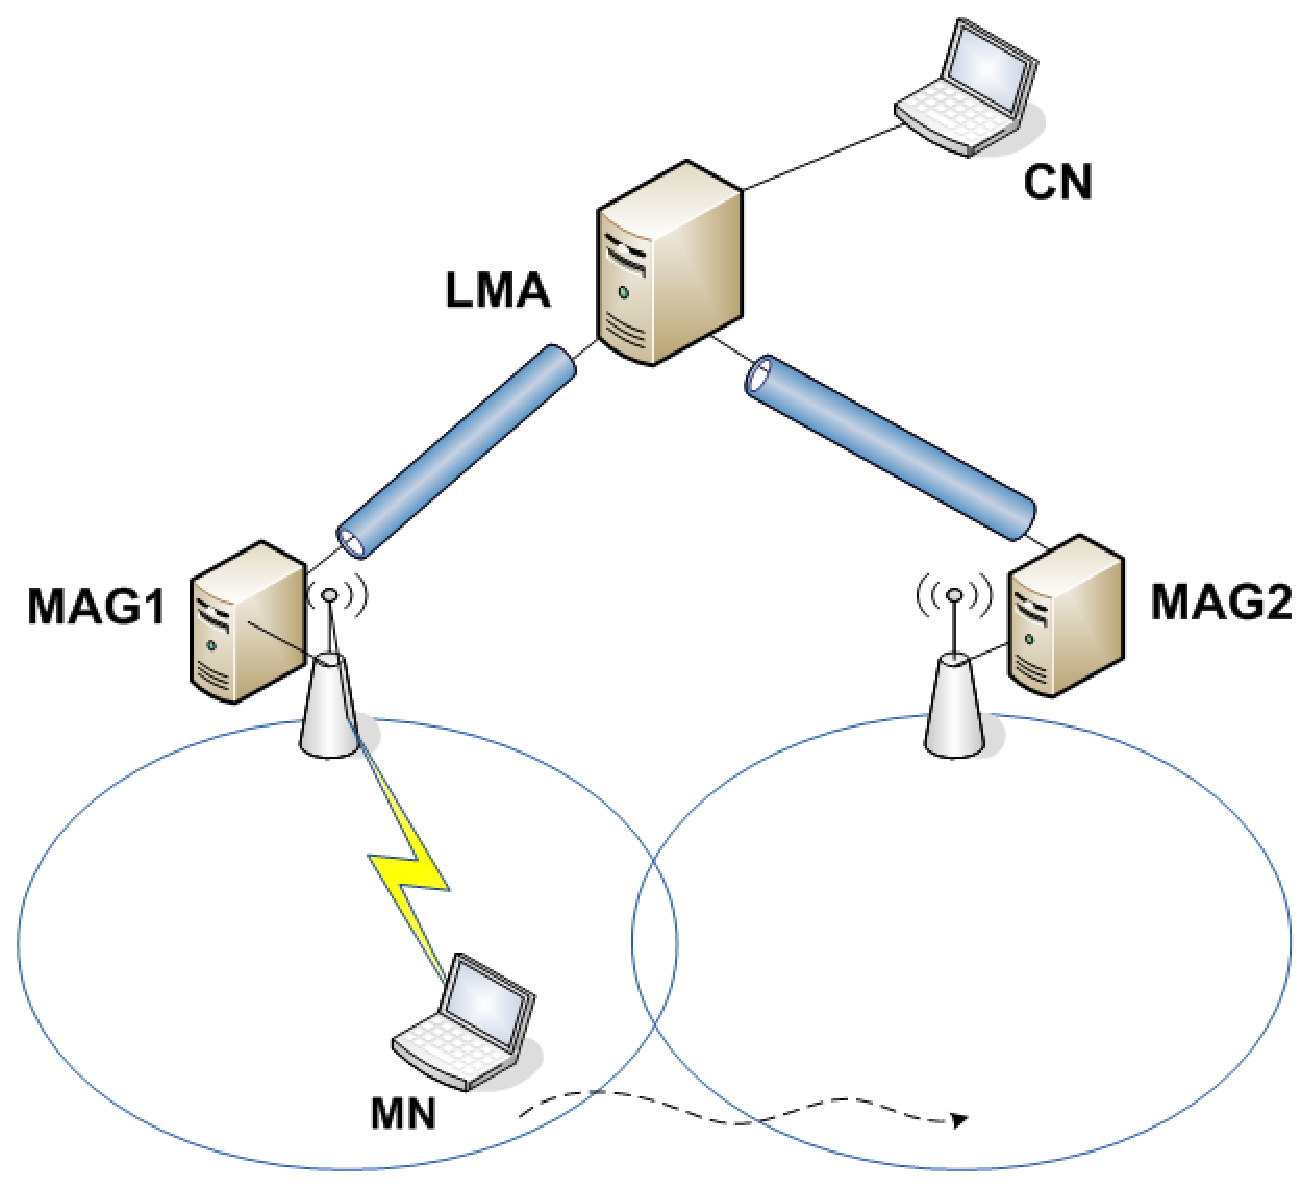
\includegraphics[width=0.4\textwidth]{./Part1/Chapter3/figures/c5_pmip_domain.eps} \label{fig:c5_pmip_domain}}\,
\subfloat[]{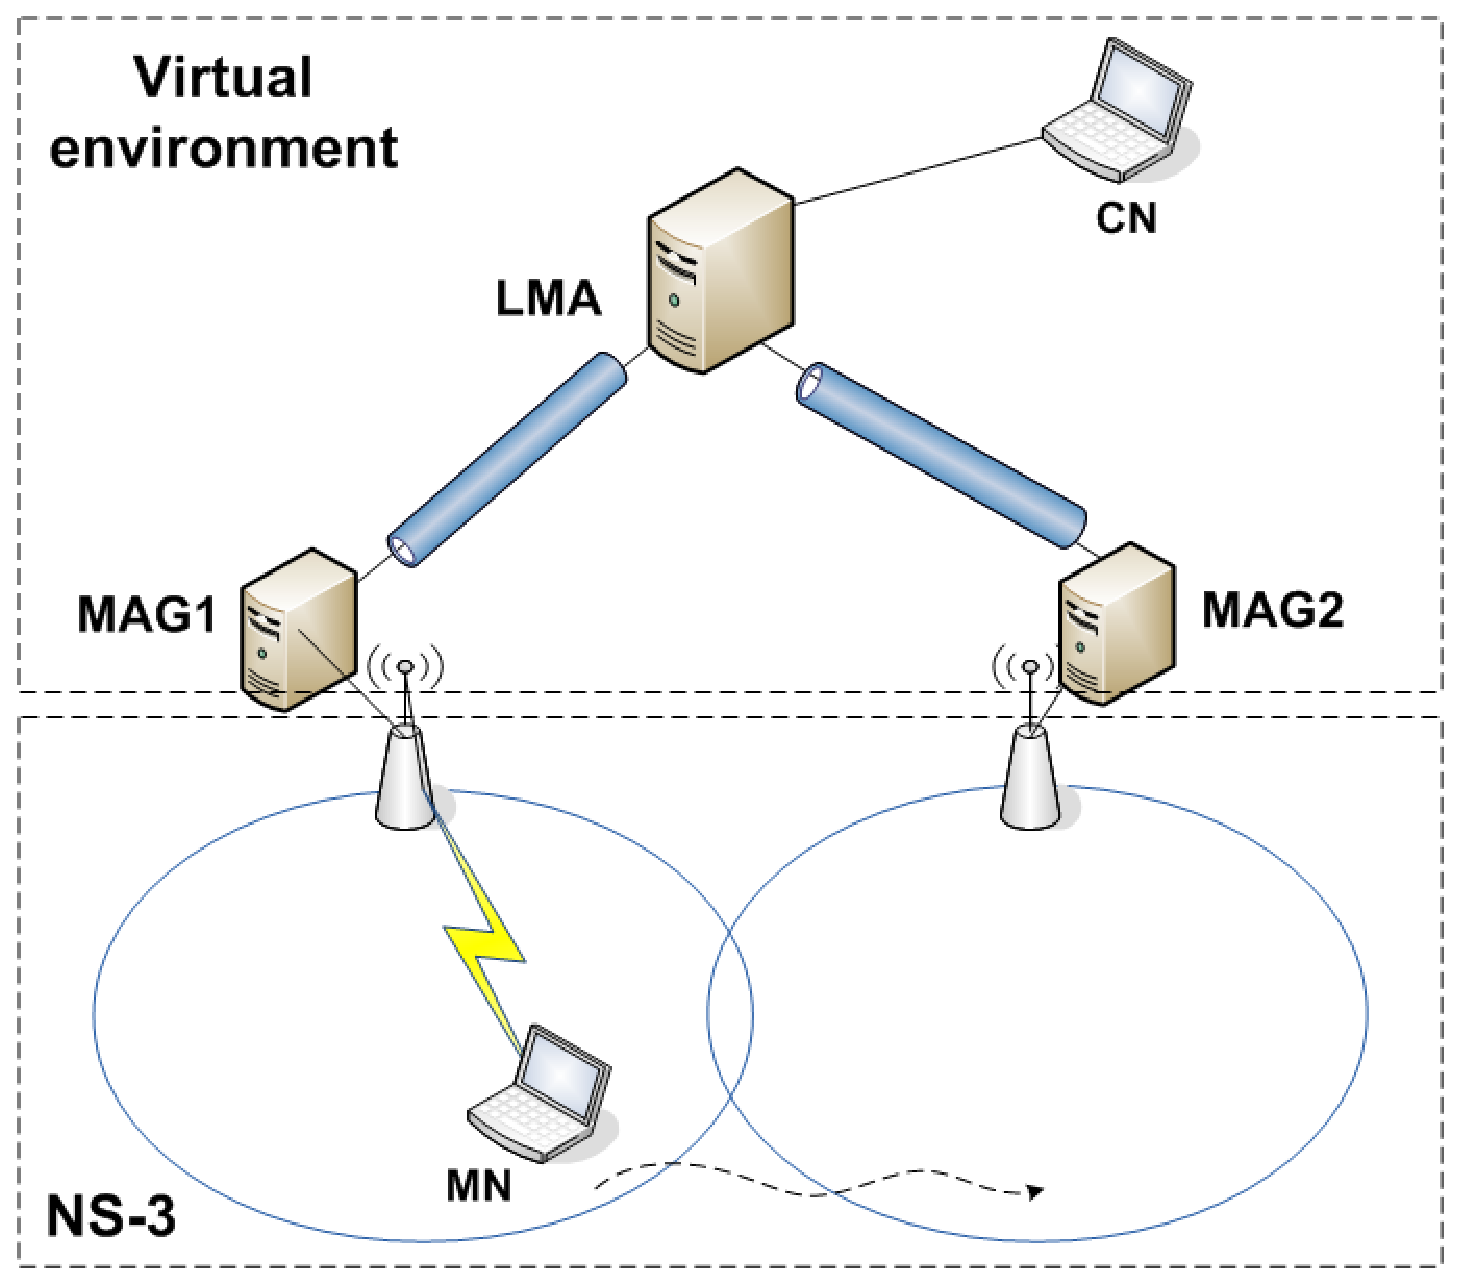
\includegraphics[width=0.4\textwidth]{./Part1/Chapter3/figures/c5_ns3_testbed.eps}\label{fig:c5_ns-3_testbed}}
\caption[The PMIP domain and the corresponding testbed.]{The PMIP domain and the corresponding testbed: (a) A PMIPv6 domain, (b) NS-3 centered testbed.}
\label{fig:scenario1}
\end{figure}

In order to validate the performance of the proposed approaches in terms of flexibility and accuracy, we present a case study in which the mobility in a PMIPv6 domain will be experimented. We will then use PMIPv6 operational behavior as benchmark to compare the experiment results from our approaches with those from a real testbed and those from pure simulation. We have carefully deployed the same PMIPv6 parameters and scenario (following the existing real testbed) in our hybrid testbeds and in the NS-3 simulator. In addition, to obtain more realistic and reliable results from the proposed testbed, we follow some guidelines to collect and analyze the results which were proposed in \cite{art_of_analysis}. 

As stated before, we have chosen to deploy our case study scenario across several platforms to demonstrate that the performance of our approaches is similar to the one provided by a real testbed. Therefore we deployed a PMIPv6 scenario containing a single MN, two MAGs connected to an LMA and a CN, as described in Fig.~\ref{fig:c5_pmip_domain}. Since mobility is not the main purpose of this chapter, for the sake of simplicity, a very basic mobility model is used: the MN moves between two MAGs with a fixed speed and a fixed direction. Later however, other mobility patterns will be applied to provide a more flexible mobility of the MN.

The experiment is executed following these steps:
\begin{itemize}
\item The MN enters the PMIPv6 domain for the first time (attaches to MAG1);
\item After configuring an IPv6 address based on the HNP allocated from the LMA, the MN uses its address to ping the CN;
\item The MN then performs a handover to move to another MAG (MAG2). During handover process, the MN continues to ping the CN.
\end{itemize}

This scenario was then tested across three different types of platform: i) a real testbed as to represent the base benchmark; ii) our NS-3 hybrid testbed; iii) NS-3 simulation. In cases (i), and (ii), we have deployed the OAI PMIPv6 implementation \cite{oai_pmip}, while in case (iv) we opted by the NS-3 embedded implementation to better show the performance difference.
\subsubsection{Different Platforms}

\paragraph{Real PMIP Testbed (R-PMIP)}
There is a real testbed \cite{oai_pmip} which was deployed in similar architecture as described in Fig.~\ref{fig:c5_pmip_domain}. All the network entities in the testbed are running Ubuntu 10.04 LTS.

\paragraph{Proposed Testbed (PMIP-NS3)}
The testbed, as indicated in Fig.~\ref{fig:c5_ns-3_testbed}, is composed of one LMA, two MAGs (and two access points (APs)), one CN and one MN. All components are installed on a single physical machine running Ubuntu 10.04 LTS. The LMA, the MAGs and the CN are the virtual machines (UML) while the MN and the APs are NS-3 nodes. It is noted that the CN is a normal UML machine that does not need any specific requirements and functionalities. The run script, which automatically launches and connects the virtual machines together, is created (one time but executed for many times). 
\paragraph{A \textit{pure-simulation PMIPv6} (Pure-NS3)}
Based on the existing PMIPv6 implementation in NS-3 (called Pure-NS3 \cite{pmip_ns3}), a simulation has been made using this implementation with the same network topology as in as well as the same result obtaining method and experiment parameters.

\subsubsection{Scalability}
Besides the comparison testing based on typical and very simple PMIPv6 case scenario, which states to the credibility of our work, we wanted also to give insight on how our proposals behave on a larger environment based on the same case study. Such analysis will demonstrate the capability to extend the range of scenario possibilities that can be researched using our developed methods as well as attest to its scalability, which is a critical, defining and differentiating feature of our work. To that aim we expanded the base case study into several scenarios comprising different topologies and a larger amount of entities, as can be seen on Fig.~\ref{fig:c5_scalability_testbed}. In order to analyze the scalability we enlarged the case study topology in both number of LMAs/MAGs and number of MNs. We first do it separately to know how the resource consumption is affected when the number of each is changed, and finally we increase both to test how far we can push our approaches.
\begin{figure}[tb!] 
  \begin{center} 
    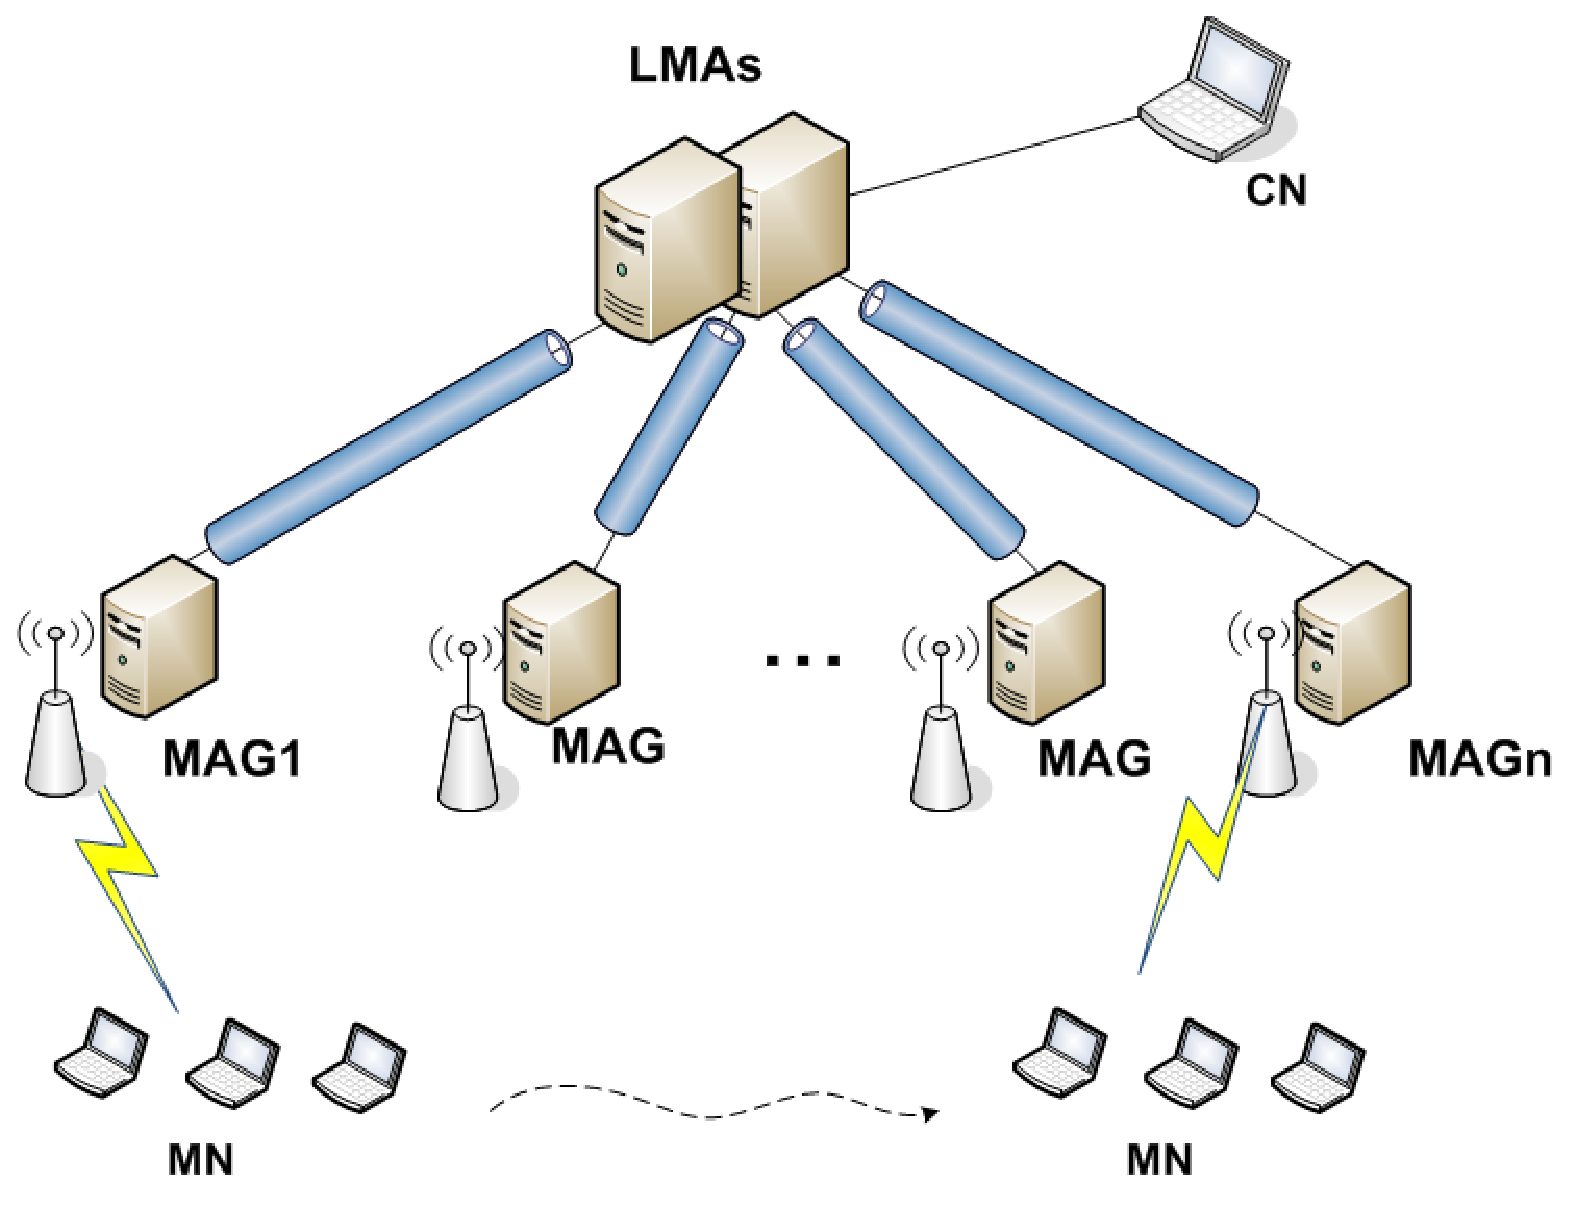
\includegraphics[width=0.45\textwidth]{./Part1/Chapter3/figures/c5_scalability_testbed.eps} 
    \caption[Illustration of the scalability tesbed.]{Scalability testbed.}
    \label{fig:c5_scalability_testbed}
  \end{center} 
\end{figure}  
\subsection{Evaluation} 
In this section, at first, we compare different approaches regarding high-level metrics and PMIP performance. We then focus on the proposed approach by measuring the resource usage in different experiment scenarios and in different steps. This section also discusses the limitation of the proposed approach regarding number of nodes and introduces some additional suggestions regarding those limitations.

Regarding the statistical evaluation and presented tables of results, it is noted that for the improvement of the credibility we performed the experiment a large amount of times. Based on the collected results, we calculate the average value and the standard deviation to improve the degree of confidence.
\subsubsection{High Level Metrics}

\begin{table}[ht!]
\footnotesize
\caption[Method of experimentation: Comparison between different approaches regarding the high level metrics.]{Comparison between Different Approaches: High Level Metrics.}
\label{tap:high_level}
\centering
\begin{tabular}{|p {5cm} |c |c |c |}%{|l|l|l|l|l|l|}%
\hline
\textbf{Metrics} & \textbf{PMIP-NS3} & \textbf{R-PMIP} & \textbf{Pure-NS3}   \\
\hline
Detecting the software and hardware requirements & Yes & Yes  &  No \\
\hline
Detecting the conflict of the components, kernel version & Yes & Yes  &  No \\
\hline
Detecting unexpected errors during runtime & Yes & Yes  &  No \\
\hline
Detecting the limitations of PMIPv6 implementation regarding number of supported nodes (MAG, MN) &Yes &Yes&No \\
\hline
Observing the actual behavior of PMIPv6 & Yes & Yes  &  Yes	 \\
\hline
Hardware cost	& Low & High & Low\\
\hline
Portability	 & Yes& Yes & No\\
\hline
\end{tabular}
\end{table}
\normalsize

When testing a new application/protocol, in some cases, it is very important to make sure that all the components can work together in a unique environment. Also, observing the interaction between these entities as well as between the components inside each entity is required to guarantee that the application/protocol can work correctly. 

Thus, while the R-PMIP and the PMIP-NS3 help to detect the software and hardware requirements, the conflict of the component as well as the unexpected errors during run-time, the Pure-NS3 cannot. To detect the limitations of PMIPv6 implementation regarding number of supported nodes (MAG and MN), our approach (PMIP-NS3) is a good choice. A real tesbed, in theory, can do the same, however, often unfeasible due to expensive cost and difficult to manage. The Pure-NS3 like the others allows observing the actual behavior of PMIPv6, however, only limited observation regarding messages exchanged between entities. Regarding hardware cost, the PMIP-NS3 and the Pure-NS3 require only one physical machine while the real testbed needs 5 physical machines, two wireless access points and one Hub. The number of required machines will be increased when a medium or large-scale experiment is considered. Another important aspect is that the PMIP implementation in our approach can be easily transfer into real word, while it requires re-develop in the Pure-NS3. 

As in the PMIP-NS3, the MNs are the NS-3 nodes, it is suitable for the experiment that does not require any specific functions/components at the MNs. Vice versa, the extra effort is needed to deploy the additional components/functionalities required in NS-3. As a result, for the experiment which does not require a lot of MNs and requires some extra functions at MNs, instead of deploying the MNs inside NS-3, we can deploy UML machines as MNs e.g., a streaming source as discussed in \cite{Thinh_Springer}. In conclusion, Table \ref{tap:high_level} summarizes the comparison of three approaches regarding different aspects. 
\subsubsection{PMIPv6 Benchmark}
Table \ref{tap:pmip_benchmark} shows the performance of PMIPv6 regarding the average value (<x>, in ms) and the standard deviation ($\sigma_{x}$) from the different approaches. Two metric are considered i.e., home address registration and layer 3 handover latency. While the former aims at showing the performance of PMIPv6 using the virtual environment, the latter is used to illustrate the performance PMIP regarding the combination of virtual and wireless environment.

In the Table \ref{tap:pmip_benchmark}, we can see that the results from the Pure-NS3 are very different from those of the PMIP-NS3. The results from the PMIP-NS3 are quite close to those from a real testbed \cite{oai_pmip}. On the contrary, the results from the Pure-NS3 environment are totally different from that of the real testbed. Thus, it is obvious that the Pure-NS3 cannot be used for the performance study of the PMIPv6 as well as the service deploying in this PMIPv6 network.\\

\small
\begin{table}[ht]
\footnotesize
\caption[PMIPv6 benchmark: Comparison between different approaches.]{Comparison between different approaches.}
\label{tap:pmip_benchmark}
\centering
\begin{tabular}{|p {5cm} |c |c |c |}%{|l|l|l|l|l|l|}%
\hline
\textbf{Metrics $<x>, \sigma_{x}$} & \textbf{R-PMIP}  & \textbf{PMIP-NS3} & \textbf{Pure-NS3}   \\
\hline
Home address registration & (3.0, 1.3) & (5.5, 1.5) & (0.1, 0)  \\
\hline
Layer 3 handover latency & (97.3, 12.3) &(110.6, 23.8) & (1.0, 0) \\
\hline
\end{tabular}
\end{table}
\normalsize

\subsubsection{Scalability Evaluation}
This subsection focuses on the PMIP-NS3 approach by measuring its resource usage regarding CPU and memory consumption depending on different stages and different configurations.

Several network topology configuration sets were defined. The sets are described in the fashion (number of LMAs, number of MAGs, number of MNs) and are constituted as follows: Conf1 (1, 3, 3), Conf2 (1, 3, 90), Conf3 (1, 10, 10), and Conf4 (1, 10, 90). The results were collected in two steps: i) step1: when the testbed is in the preparing mode (after the booting of all virtual machines and their required components; and ii) step 2: the testbed is in the running mode (when MNs attaches and performs handover inside the domain). During the experiment, the processors and the memory related statistics were collected each one second during 100 seconds to improve the credibility. It was done by using some tools e.g., mpstat and top. We also measure the “background processes” (BP) by using the same mechanism.

For instance, we can deploy a PMIPv6 domain with up to one LMA, 10 MAGs, one CN, and one MN (all of them are virtual machines) on a single physical machine even with a very limited capacity: CPU Intel Core 2 Duo T7500 (2.2 GHz), 2 GB of RAM (1066MHz) and a 320 GB HDD running Ubuntu 10.04 LTS. By using NS-3, this testbed can support up to 90 MNs (NS-3 nodes) which can move at the same time. 

\begin{figure}[h!]
\centering
\subfloat[]{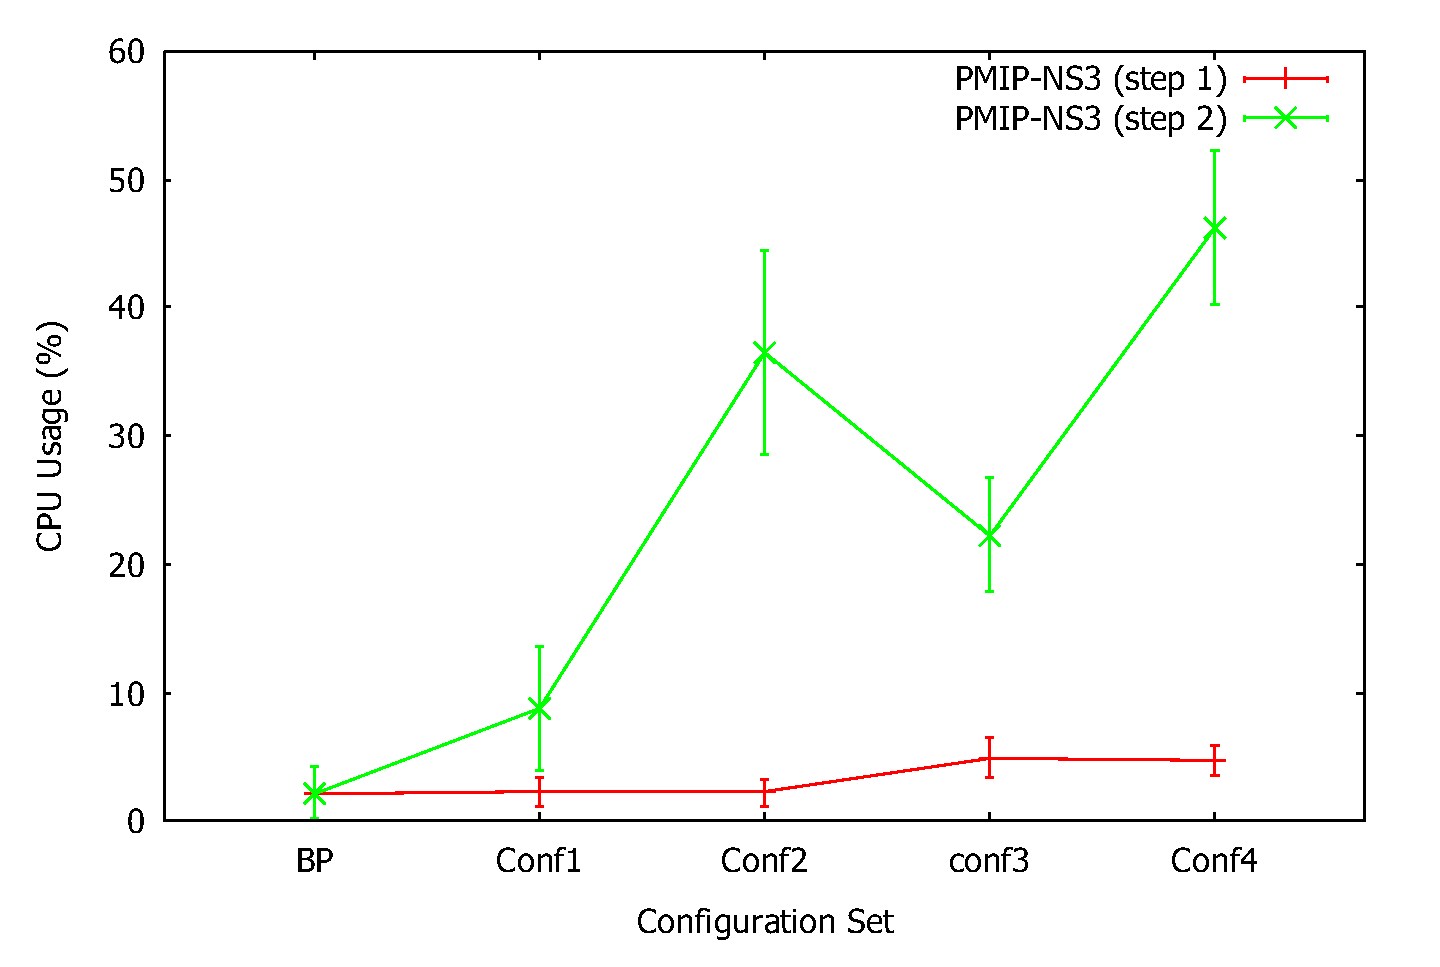
\includegraphics[width=0.47\textwidth]{./Part1/Chapter3/figures/c5_cpu_usage.eps} \label{fig:c5_cpu_usage}}\,
\subfloat[]{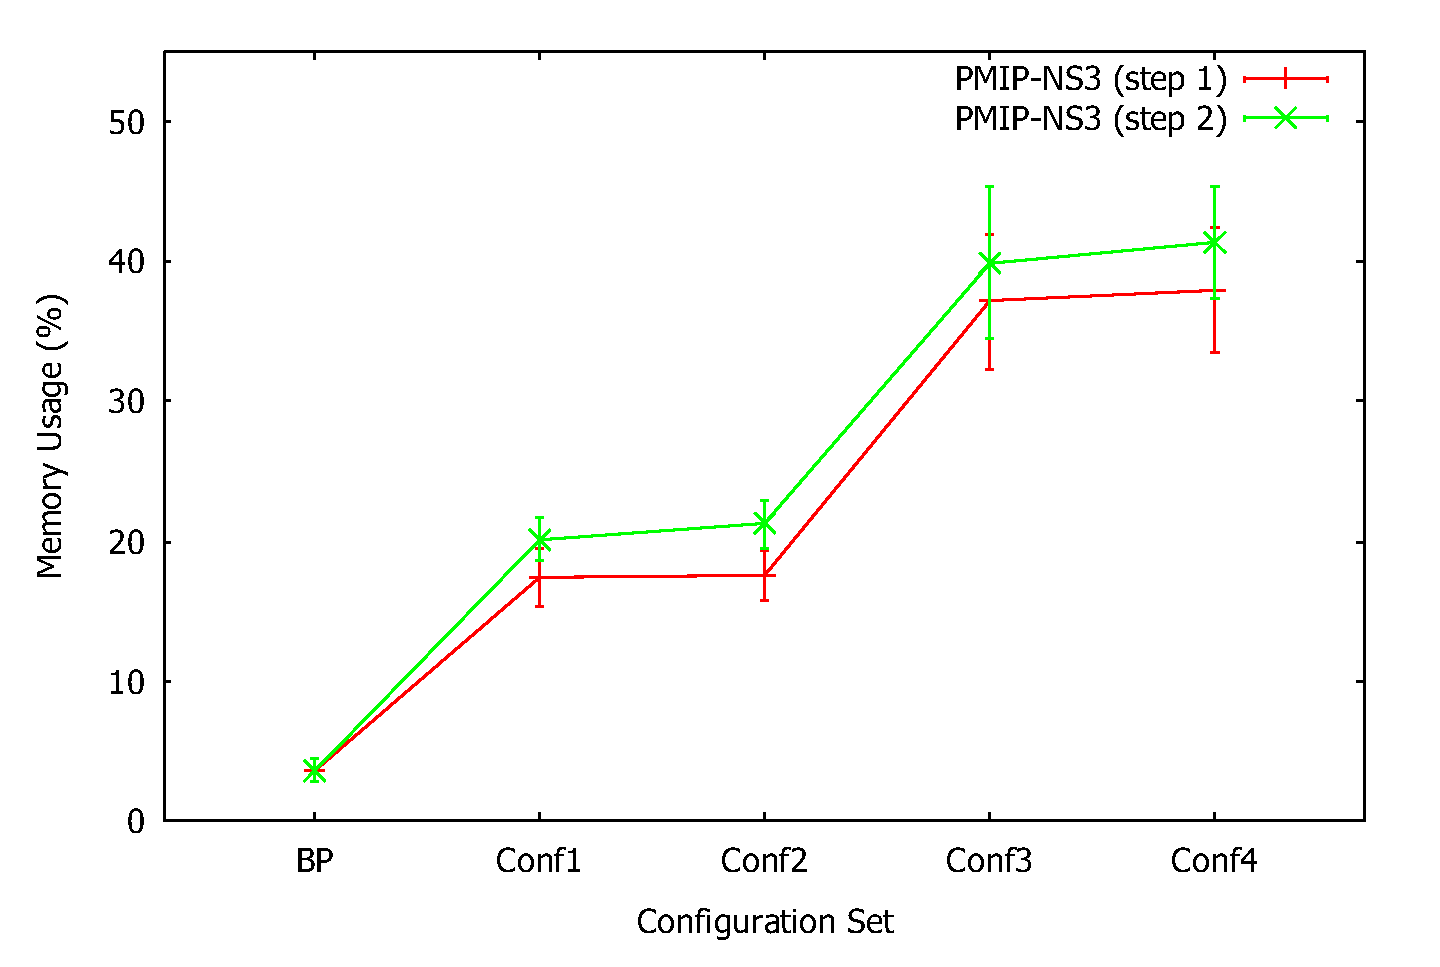
\includegraphics[width=0.47\textwidth]{./Part1/Chapter3/figures/c5_memory_usage.eps}\label{fig:c5_memory_usage}}
\caption[Resource usage of the near-to-real testbed.]{Resource usage: a) CPU, b) Memory.}
\label{fig:c5_resource_usage}
\end{figure}

The CPU and the memory consumption in the PMIP-NS3 are illustrated in Fig.~\ref{fig:c5_cpu_usage} and Fig.~\ref{fig:c5_memory_usage}, respectively. As we can observe in Fig.~\ref{fig:c5_memory_usage}, the memory consumption in the configuration 1 and the configuration 2 are almost the same. That means with the same number of virtual machines, increasing number of mobile nodes inside NS-3 does not add much more resources. On the contrary, the CPU consumption (see Fig.~\ref{fig:c5_cpu_usage},) is totally different. It is because the LMA and MAGs have to process PBU/PBA message from a lot of MNs. Also, the CPU required by NS-3 is increased. The same thing happens in case of the configuration 3 and the configuration 4.

In general, host memory/CPU is often the factor limiting the number of virtual machines that a host can support. Moreover, since many virtual machines are deployed in a single real machine, the host machine is easy to become overloaded. It influences the overall testbed especially in performance experiment. In our experiment, the memory and CPU consumption in the worst case is around 41 and 46 percent, respectively. These values seem not too high, however, it can be considered as a trade-off between the number of deployed nodes and the performance of the system (during peak period, it may consume up to 69.65\% CPU, 80.07\% memory). 

\subsubsection{Distributed Experiment Environment}

\begin{figure}[h!]
\centering
\subfloat[]{\includegraphics[width=0.485\textwidth]{./Part1/Chapter3/figures/c5_distributed_machines.eps} \label{fig:c5_distributed_machines}}\,
\subfloat[]{\includegraphics[width=0.455\textwidth]{./Part1/Chapter3/figures/c5_distributed_machines_2.eps}\label{fig:c5_distributed_machines_2}}
\caption[Near-to-real testbed: An example of the distributed experiment environment.]{An example of distribution technique.}
\label{fig:c5_distributed_machine}
\end{figure}

In the experiment described in the previous subsection, the testbed can support up to 10 MAGs and 90MNs. While it is suitable for a medium scale experiment, it is not enough for a large scale one. The number of supported nodes is limited since the experiment environment is realized on a single machine which has limited resources. Some of them are consumed by the virtual machines, and some are by the simulator NS-3.

To overcome this limitation, the testbed can be deployed in a distributed manner among different physical machines. There are several methods to deploy the proposed testbed in a distributed way. The first method divides the network into several sub networks in which each sub network is deployed in a single host machine. For example, in Fig.~\ref{fig:c5_distributed_machines}, a PMIPv6 domain deployed at the real machine 1 is extended by implementing the extra LMAs, MAGs in different real machines (machine 2, 3, 4). 

To illustrate this method, we deployed a testbed in two different physical machines. A PMIPv6 domain has been deployed in the first real machine similar to in the previous section (testbed in a single machine). Some MAGs then have been installed in the second machine. As a result, we can deploy a network with two LMAs, 21 MAGs and 150 MNs. However, one limitation is that the PMIPv6 domain is divided into different \textit{sub networks} (in different computers) in which the MN cannot move between sub networks. Some extra techniques should be applied to allow the MN to move between different real hosts such as MPI for distributed simulation \cite{MPI}. Another method addresses this limitation by putting the wireless environment in only one physical machine as described in Fig.~\ref{fig:c5_distributed_machines_2}. In this case, the tunneling mechanism is required to connect multiple MAGs with their APs via only one interface. However, it raises some other issues as mentioned in \cite{limitation_single_machine}. 

\section{Conclusion}
This chapter at first gives the performance metrics which are crucial to evaluate a proposal for IP mobility management as well as IP mobile multicast. These metrics are then presented in details from a mathematical point of view. Next, we discuss different methods of experimentation for wireless mobile networks. We argue that, the most widely used method – simulation – sometimes lacks credibility in produced results, which is a critical issue for solution deployment. Furthermore, the use of real testbeds can obtain more reliable results, though they are much more costly and only built in a small scale. We then introduce a hybrid method which is a combination of virtualization and simulation. Through the study of a simple use-case showing mobility with PMIPv6, we demonstrate that our proposed method provides realistic results at a low cost. In other words, the near-to-real results can be achieved even with limited resources by using the proposed method.  Additionally, this method can be deployed in a distributed manner for increased scalability.

As in our proposed testbed, the MNs are the NS-3 nodes, thus, it is suitable for the experiment that does not require any specific functions/components at the MNs. Vice versa, the extra effort is needed to deploy the additional components/functionality required in NS-3. As a result, for the experiment which does not require a lot of MNs and requires some extra functions at MNs, instead of deploying the MNs inside NS-3, we can deploy UML machines as MNs e.g., streaming source. This scenario is described in \cite{Thinh_Springer}. In addition, in some cases, real wireless/wired environment should be provided. A real machine can be used as an MN, while the network entities are deployed in another computer similar to in \cite{PMIP_EV}.

In order to validate a multicast solution in a mobile environment, the experimental results should be provided with high degree of confidence. In this context, our proposed testbed is basically suitable for measuring such performance metrics as multicast service disruption and packet loss, end-to-end delay and load balancing (scalability) when mathematical model is suitable for signaling and packet delivery cost, packet duplication and tunneling overhead.  






